%
% business_plan.tex
%
% Copyright © 2016 Franco Masotti <franco.masotti@student.unife.it>
% This work is free. You can redistribute it and/or modify it under the
% terms of the Do What The Fuck You Want To Public License, Version 2,
% as published by Sam Hocevar. See the LICENSE file for more details.
%

\documentclass{beamer}
\usepackage{graphicx}
\usepackage[gen]{eurosym}
\usetheme{Warsaw}
\title{3DFePrint}
\subtitle{Business plan high-tech}
\author{Franco Masotti}
\date{\today}
\hypersetup{pdfstartview={Fit}}
\begin{document}

    \frame{\titlepage}

    \begin{frame}
        \frametitle{Origini dell'azienda}
            \begin{itemize}
                \item L'impresa nasce dall'idea di creare piccoli oggetti di 
uso quotidiano e di prototipazione attraverso la tecnologia di stampa 3D 
desktop.
                \item La mission della nostra startup \'e di fare in modo che 
chiunque possa ottenere gli oggetti che desidera in modo semplice ed 
economico, pur mantenendo la massima qualit\'a possibile.
                \item Siamo in 8 persone tra tecnici, grafici, programmatori 
web e contabili.
                \item I nostri prodotti sono rivolti sopratutto a privati ed a  
piccole industrie (ad esempio per la prototipazione). Saremo anche disponibili 
per consulenze riguardanti la stampa 3D in generale (setup, corsi, etc...).
            \end{itemize}
    \end{frame}

    % Compagine
    \begin{frame}
        \frametitle{Composizione e forma giuridica}
            \begin{itemize}
                \item La nostra impresa \'e composta da 8 persone:
                \begin{itemize}
                    \item 2 grafici
                    \item 1 addetto ai sistemi
                    \item 2 programmatore web
                    \item 1 Addetto marketing e pubblicit\'a
                    \item 1 contabile e addetto alla amministrazione
                    \item 1 responsabile
                \end{itemize}
                \item Siamo una startup \emph{S.A.S.} localizzata a Ferrara.
            \end{itemize}
    \end{frame}

    % Output
    \begin{frame}
        \frametitle{Breve descrizione del processo produttivo e interazione con il cliente}
            \begin{itemize}
                \item I disegni degli oggetti (\emph{CAD}) vengono inviati dai
clienti attraverso una piattaforma web.
                \item L'utente ha la possibilit\'a di creare i progetti 
direttamente dal sito assemblando componenti note, oppure di inviare disegni 
totalmente nuovi.
                \item A discrezione dell'utente, una volta che i progetti sono 
stati inviati, vengono salvati e resi disponibili a tutti (attraverso la 
piattaforma) grazie alla licenza \emph{CC BY-SA}, che permette la modifica e la 
ridistribuzione dei progetti, anche per scopi commerciali.
                \item L'utente sceglie il tipo/i di materiale con cui deve 
essere stampato l'oggetto.
                \item Una volta completato il prodotto, questo viene spedito 
per posta, in tutto il mondo, oppure pu\'o essere ritirato direttamente dalla 
sede.
            \end{itemize}
    \end{frame}

    \begin{frame}
        \frametitle{Mantenimento vantaggi competitivi}
            \begin{itemize}
                \item Per mantenere il vantaggio competitivo, svilupperemo 
la progettazione del software e dell'hardware delle stampanti nel corso del 
tempo, in base alle esigenze e all'evoluzione del mercato.
                \item Questi due obbiettivi sono possibili visto che si tratta 
di \emph{software libero} ed \emph{open hardware} (si ha la 
possibilit\'a di studiare, modificare e ridistribuire il software e 
l'hardware per qualunque scopo). Per farlo, assumeremo personale altamente 
qualificato.
                \item Successivamente, una volta che avremo acquisito 
esperienza, entreremo anche nel settore della scansione 3D, che si andr\'a ad 
integrare con la stampa 3D. Anche in questo caso non useremo tecnologia 
proprietaria.
            \end{itemize}
    \end{frame}

    \begin{frame}
        \frametitle{Comunit\'a}
            \begin{itemize}
                \item Il fatto che utilizzeremo software libero e open hardware 
ci permetter\'a di creare una comunit\'a di utenti ed entusiasti dei nostri 
prodotti e servizi.
                \item Questo succede gi\'a con imprese simili (tra le pi\'u 
famose \emph{OwnCloud}, \emph{Raspberry}, \emph{Ubuntu} e molte altre) che 
riescono a promuoversi grazie a forum, mailing list, conferenze specializzate 
e molti altri eventi.
            \end{itemize}
    \end{frame}

    % Ambiente competitivo
    \begin{frame}
        \frametitle{Concorrenti}
            \begin{itemize}
            \item Nella nostra zona esistono alcuni concorrenti, ad esempio: 
\emph{Computer Facile} e \emph{Next Informatica}.
            \item I concorrenti, non essendo specializzati per la stampa 3D, 
non hanno un alto volume di affari per quanto riguarda questo settore. Inoltre 
non dispongono dell'interfaccia web citata precedentemente.
            \end{itemize}
    \end{frame}

    \begin{frame}
        \frametitle{Partner commerciali}
            \begin{itemize}
                \item \emph{Librebot} ci fornisce le stampanti ed i filamenti. 
Li contatteremo direttamente per fare un accordo in modo da ottenere 
sconti per quanto riguarda i materiali di stampa.
                \item \emph{ThinkGnu} ci fornisce i computer e tutto il 
materiale informatico necessario.
                \item Prenderemo anche accordi con corrieri.
            \end{itemize}
    \end{frame}

    \begin{frame}
        \frametitle{Strategie di mercato}
        \begin{itemize}
                \item Il prezzo di ogni manufatto sar\'a determinato dal tempo 
di stampa, dal tipo e dalla quantit\'a di materiale/i utilizzato/i.
                \item Per ci\'o che riguarda il marketing punteremo molto sulla 
pubblicit\'a via web, in particolare con i social network. 
Per i primi mesi di attivit\'a, perch\'e il mercato inizi a conoscerci, 
utilizzeremo publicit\'a su radio e giornali.
                \item Ci concentreremo principalmente sulla vendita via 
Internet dando ai clienti molteplici possibilit\'a di pagamento, da quelle 
tradizionali alla cryptocurrency (Bitcoin, etc...). Il cliente potr\'a anche 
scegliere varie modalit\'a di spedizione.
        \end{itemize}
    \end{frame}

    % Organizzazione aziendale.
    \begin{frame}
        \frametitle{Localizzazione dell'azienda}
            \begin{figure}[H]
               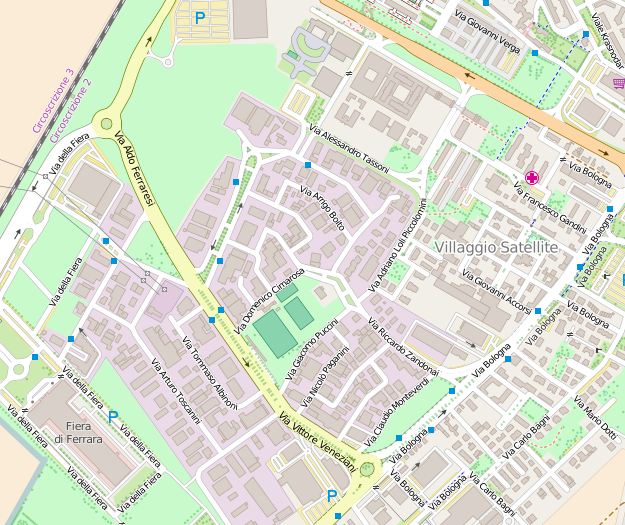
\includegraphics[scale=0.15]{map.png}
                \caption{\copyright{} OpenStreetMap contributors, Open 
Database License, CC BY-SA}
            \end{figure}
            \begin{itemize}
                \item Ci troviamo nella zona \emph{P.M.I} di Ferrara.
                \item Abbiamo scelto questa citt\'a perch\'e dispone di 
un discreto numero di attivit\'a interessate ai nostri prodotti. Attualmente 
ci sono pochi concorrenti commerciali nella zona.
                \item La sede \'e facile da raggiungere dalle principali reti 
stradali.
            \end{itemize}
    \end{frame}

    \begin{frame}
        \frametitle{Investimenti}
            \begin{table}[h]
                \begin{tabular}{lrrr}
                    \hline
                    \multicolumn{4}{c}{\textbf{Piano investimenti}} \\
                    \cline{1-4}
                    Investimento & Anno I (\euro{}) & Anno II (\euro{}) & Anno 
III (\euro{}) \\  \hline
                    Adeguamento fabbricato & 15000 & 0 & 0 \\
                    Stampanti 3D & 7500 & 5000 & 2500 \\
                    Computer e accessori & 8000 & 3000 & 1000 \\
                    Piattaforma web & 4000  & 2000  & 500  \\ \hline
                    Totali & 34500  & 10000  & 4000  \\ 
                    \hline
                \end{tabular}
                \caption{Piano degli investimenti nel corso dei primi tre 
anni}
            \end{table}
            \begin{itemize}
                \item Ogni stampante ha un costo di 2500 \euro{}
                \item Si prevede quindi un investimento minimo di circa 48500
\euro{} nel corso dei primi tre anni. 
            \end{itemize}
    \end{frame}

    % Piano economico finanziario
    \begin{frame}
        \frametitle{Costi}
            \begin{table}[h]
                \begin{tabular}{lr}
                    \hline
                    \multicolumn{2}{c}{\textbf{Piano costi}} \\
                    \cline{1-2}
                    Costo & Quantit\'a (\euro{}) \\  \hline
                    Affitto fabbricato & 12000 \\
                    Stipendi e contributi & 144000 \\ 
                    Spese di mantenimento (bollette, etc...) & 8000 \\ \hline
                    Totale & 164000 \\
                    \hline
                \end{tabular}
                \caption{Piano dei costi annuale}
            \end{table}
            \begin{itemize}
                \item Un costo variabile sar\'a l'acquisto dei filamenti 
(i materiali per la stampa), calcolato in base agli ordini.
                \item Tutto il processo produttivo viene completato con 
software libero, in modo da abbattere i costi. Questo si 
verifica in quanto si evita l'acquisto di licenze per l'utilizzo del 
software. Ci sar\'a inoltre supporto da una comunit\'a di sviluppatori 
interessati al progetto.
            \end{itemize}
    \end{frame}

    \begin{frame}
        \frametitle{Previsioni di fatturato}
            \begin{table}[h]
                \begin{tabular}{lrrr}
                    \hline
                    \multicolumn{4}{c}{\textbf{Fatturato piccoli oggetti}} \\
                    \cline{1-4}
                    & Anno I & Anno II & Anno III \\ \hline
                    Volume & 6000 & 9000 & 9000 \\
                    Prezzo medio unitario (\euro{}) & 200 & 180 & 180 \\ 
                    \hline
                    \multicolumn{4}{c}{\textbf{Fatturato prototipazione}} \\
                    \cline{1-4}
                    Volume & 1500 & 3000 & 4500 \\
                    Prezzo medio unitario (\euro{}) & 500 & 450 & 420 \\
                    \hline
                    \multicolumn{4}{c}{\textbf{Totali (\euro{})}} \\
                    \cline{1-4}
                    & 1950000 & 2970000 & 3510000 \\
                    \hline
                \end{tabular}
                \caption{Previsioni di \textbf{massimo} fatturato nel corso dei 
primi tre anni.}
            \end{table}
            \begin{itemize}
                \item In media ogni stampante produce 10 piccoli oggetti oppure 
5 prototipi al giorno. Ogni anno lavorativo viene considerato di 300 giorni.
                \item Nei primi tre anni di attivit\'a prevediamo circa 
8430000 \euro{} di fatturato.
            \end{itemize}
    \end{frame}

    \begin{frame}
        \frametitle{Punto di pareggio}
            \begin{itemize}
                \item Costi Fissi = 164000 \euro{}
                \item Prezzo medio unitario (1950000 \euro{}/7500 pcs) = 260 \euro{}
                \item Costo variabile medio unitario = 240 \euro{}
                \item Quindi per raggiungere il punto di pareggio sar\'a 
necessaria la vendita di almeno 8200 unit\'a, prodotte a 
pieno regime. Poich\'e nel primo anno saranno prodotte 6000+1500=7500 unit\'a, 
il punto di pareggio sar\'a raggiunto dopo questo periodo di tempo.
                \item Inoltre, per il primo anno il disavanzo sar\'a di: 
(1950000-1800000)-164000 = 14000 \euro{}
            \end{itemize}            
    \end{frame}

    % Analisi conclusiva dei vantaggi competitivi e dei fattori di rischio 
    % dell'iniziativa
    \begin{frame}
        \frametitle{Rischi}
            \begin{itemize}
                \item Pur essendo un settore di mercato relativamente nuovo, 
questo tipo  di stampante sta diventando sempre pi\'u economico e facile da 
usare. Per non essere esclusi dal mercato, noi punteremo su una costante 
innovazione, sulla semplicit\'a d'uso e sulla qualit\'a dei nostri prodotti.
                \item Ci anche aspettiamo nuovi concorrenti, specialmente dai 
mercati orientali, si che possono permettere di impostare prezzi pi\'u bassi a 
causa del minor costo delle materie prime usate per la stampa, non tanto per la 
manodopera.
            \end{itemize}
    \end{frame}
\end{document}
